\documentclass[a4paper,10pt]{jsarticle}
\renewcommand{\figurename}{Fig.}
\renewcommand{\tablename}{Table }
\usepackage[left=2cm,right=2cm,top=3cm,bottom=3cm]{geometry}
\usepackage{multicol}
\usepackage{blindtext}
\usepackage{amsmath,amsfonts}
\usepackage{amssymb}
\usepackage{bm}
\usepackage{siunitx}
\usepackage[dvipdfmx]{graphicx}
\usepackage{booktabs}
\usepackage{multirow}
\usepackage{here}
\usepackage{wrapfig}
\usepackage{siunitx}

\setlength{\columnsep}{10mm}
\makeatletter
\newenvironment{tablehere}
{\def\@captype{table}}
{}
\newenvironment{figurehere}
{\def\@captype{figure}}
{}
\makeatother

\begin{document}
\title{{顕微鏡によるブラウン運動の観察と拡散係数の導出}}
\author{Teduka Yuuki 1522063 
\\
Collaborator:Nakamura Kouta 1522B02 }
\date{Lab date: 5th and 12th October 2022}
\maketitle

\begin{abstract}
この実験の目的は、ブラウン運動をする粒子の動画像を撮影し、画像解析から平均二乗変位を得ること
で粒子の拡散係数を求めることである。その後、粘性率と温度を既知としてアインシュタイン・ス
トークスの関係式よりボルツマン定数を求めることを目的とする。\\
実験では、実体顕微鏡を用いて、15\%PEG水溶液中、30\%PEG水溶液中、純水中に散乱するポリスチレン粒子の動画像を撮影した。
その結果、μmサイズの粒子が示すブラウン運動を観察できた。

\end{abstract}

\section{\textrm{Introduction}}
\section{\textrm{Theoretical background}}
\section{\textrm{Experimental procedures}}
(使用器具)\\
顕微鏡、USB カメラ、PC、スライドガラス、カバーガラス、両面テープ、メカニカル
ピペット、対物マイクロメーター\\
 (試料)\\
ポリスチレン粒子(直径0.75 μm)を純水、濃度15\%, 30\%のPEG 水溶液に分散させたも
の。\\粘性率はそれぞれ、純水:$8.9\times 10^{-4}$Pa、PEG15\%:$1.7\times 10^{-2}$Pa、
PEG30\%:$5.9\times 10^{-2}$Paである。\\
 (実験手順)\\
スライドガラスに両面テープで少し隙間を与えながら囲いを作り、そこにカバーガ
ラスをつけた。その後、囲いの隙間にメカニカルピペットを用いることで溶液を注入
し、スライドガラスを顕微鏡にセットして測定できるようにした。3 種類の溶液全て
でこの手順を行なった。ここまでできたら、顕微鏡とPC を接続し、パソコンの画面
上で顕微鏡を見ることができるようにし、両面テープの箇所を見ることで倍率の調整
を行い、溶液内のブラウン運動する粒子を捜索した。
ブラウン運動する粒子が見つかったらそれをパソコンで録画し、その動画データ
を、ソフトを用いて解析することで粒子の位置データを求めた。\\
スライドガラス内には、溶液を注入したことにより微小な流れが発生する。その流れの影響を無視するため、
2つの粒子の位置を追跡し、片方の粒子を基準としてもう片方の粒子の位置を相対座標として求めた。
マイクロメーターの画像から実際の長さを求めて距離に換算し、動画のfps から時間ごとの動きに書き換えた。これらの書き換えたデータを元に、pythonでMSDを求めた。\\
\section{\textrm{Results}}
顕微鏡で同倍率時のマイクロメーターの画像を撮影したところ、1162pxで100μmであった。この縮尺より、pxをμmに変換した。
また、撮影したカメラのfpsは、10fpsであった。これより、フレーム数を時間に変換した。

\begin{figurehere}
\centering
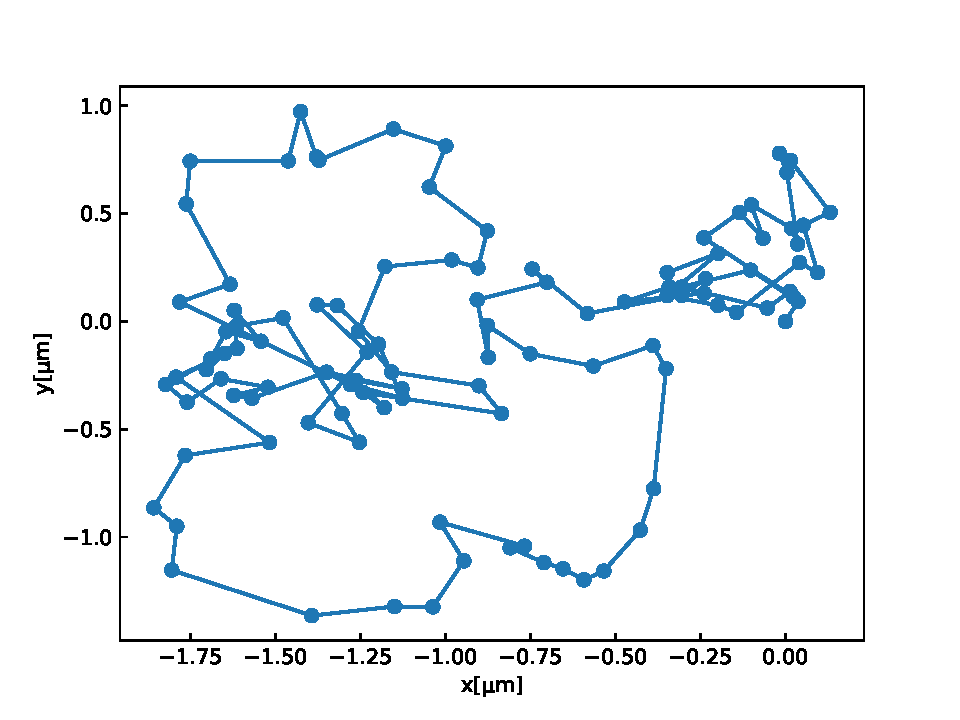
\includegraphics[width=0.7\linewidth]{fig/1_move_plot.pdf}
\caption{Movement of particles in 15\% PEG}
\label{fig:move_plot}
\end{figurehere}

PEG15\%の粒子1を相対座標とした粒子2の軌跡をFig.1に示した。\\
粒子は、左下に移動しているように見えるが、不規則に運動し、ブラウン運動をしていることが確認できた。

\begin{figurehere}
  \centering
  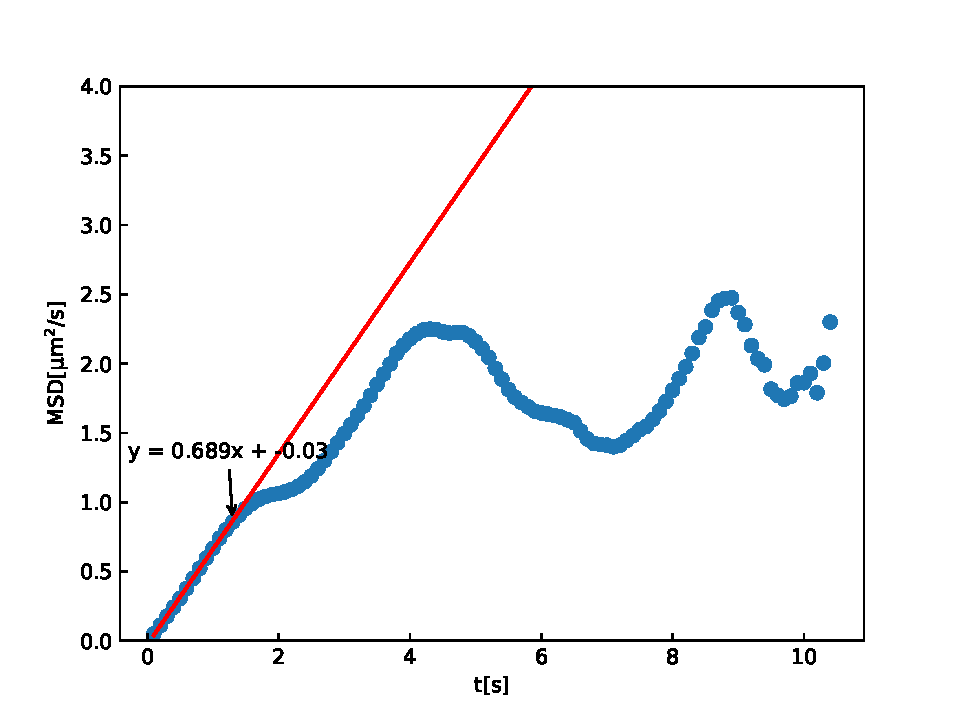
\includegraphics[width=0.7\linewidth]{fig/1_D.pdf}
  \caption{Time variation of MSD of particles in 15\% PEG}
  \label{fig:move_plot}
  \end{figurehere}

続いて、Fig.2にPEG15\%のMSDの時間依存性を示した。\\
0〜1.8s近辺の間は、線形的に増加している。この時の傾きを求めると、$0.689 \text{μm}^2/\text{s}^2$となった。\\
これより、÷8をして拡散係数を求めると、$8.64×10^{-14} \text{m}^2/\text{s}^2$となった。\\

\begin{figurehere}
\centering
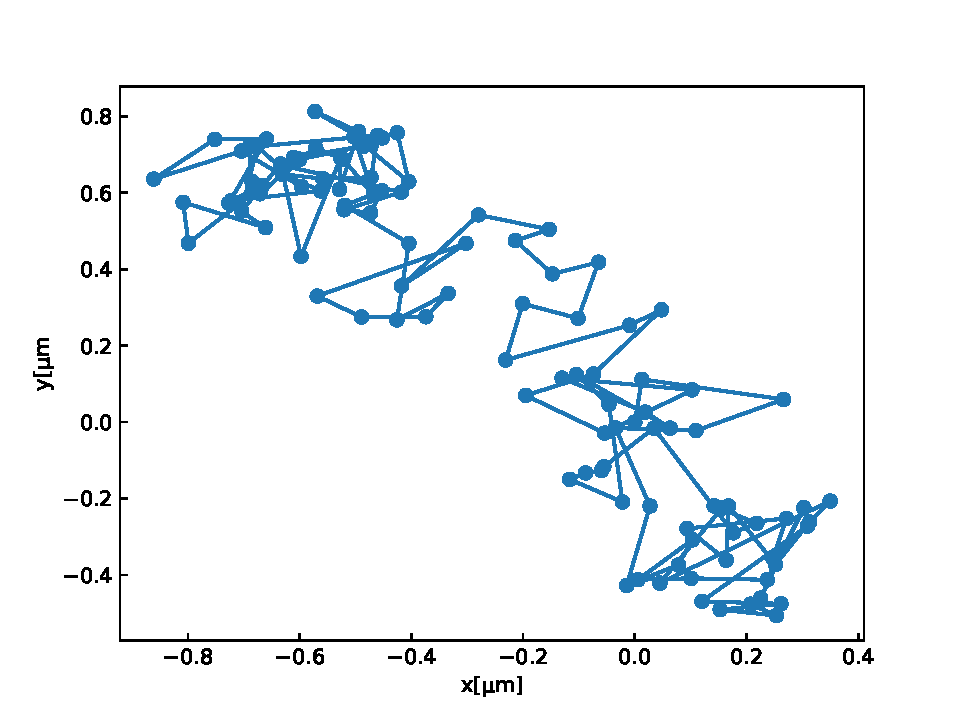
\includegraphics[width=0.7\linewidth]{fig/2_move_plot.pdf}
\caption{Movement of particles in 30\% PEG}
\label{fig:move_plot}
\end{figurehere}

PEG30\%の粒子1を相対座標とした粒子2の軌跡をFig.3に示した。\\

\begin{figurehere}
  \centering
  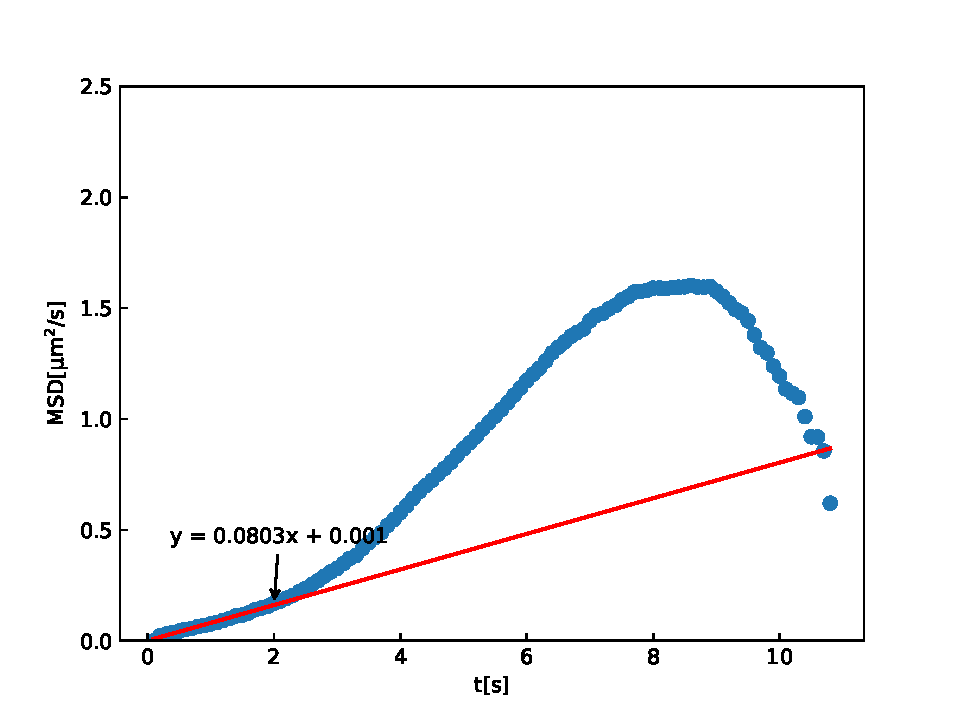
\includegraphics[width=0.7\linewidth]{fig/2_D.pdf}
  \caption{Time variation of MSD of particles in 30\% PEG}
  \label{fig:move_plot}
  \end{figurehere}

  続いて、Fig.4にPEG15\%のMSDの時間依存性を示した。\\
  0〜2s近辺の間は、線形的に増加している。この時の傾きを求めると、$0.0803 \text{μm}^2/\text{s}^2$となった。\\
  これより、÷8をして拡散係数を求めると、$1.00×10^{-14} \text{m}^2/\text{s}^2$となった。\\

\begin{figurehere}
\centering
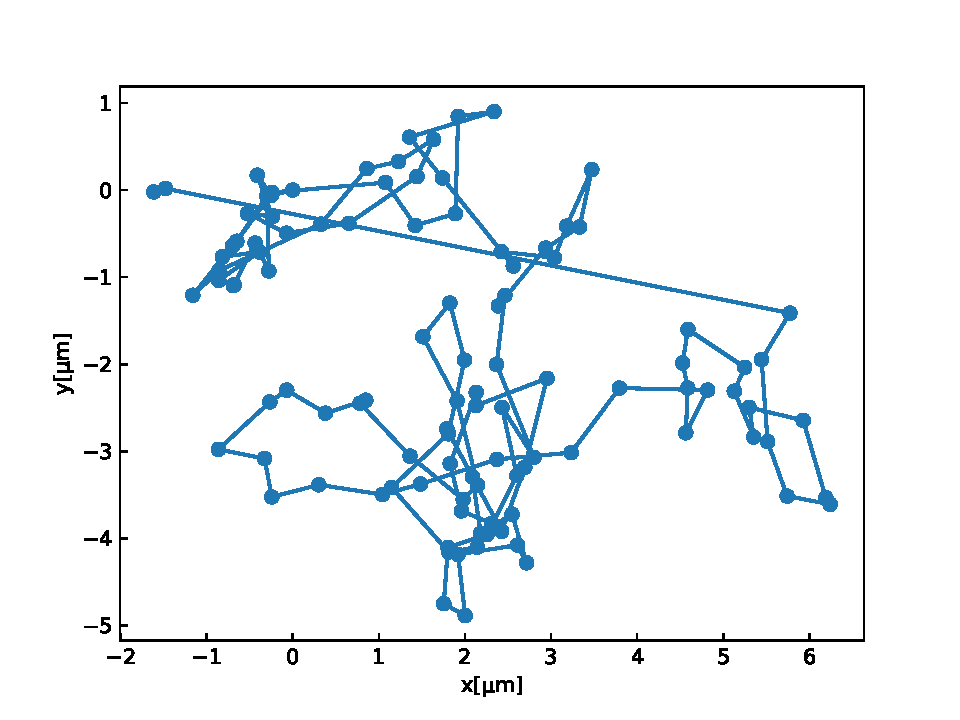
\includegraphics[width=0.7\linewidth]{fig/water_move_plot.pdf}
\caption{Movement of particles in pure water}
\label{fig:move_plot}
\end{figurehere}

純水溶液中の粒子1を相対座標とした粒子2の軌跡をFig.3に示した。\\

\begin{figurehere}
  \centering
  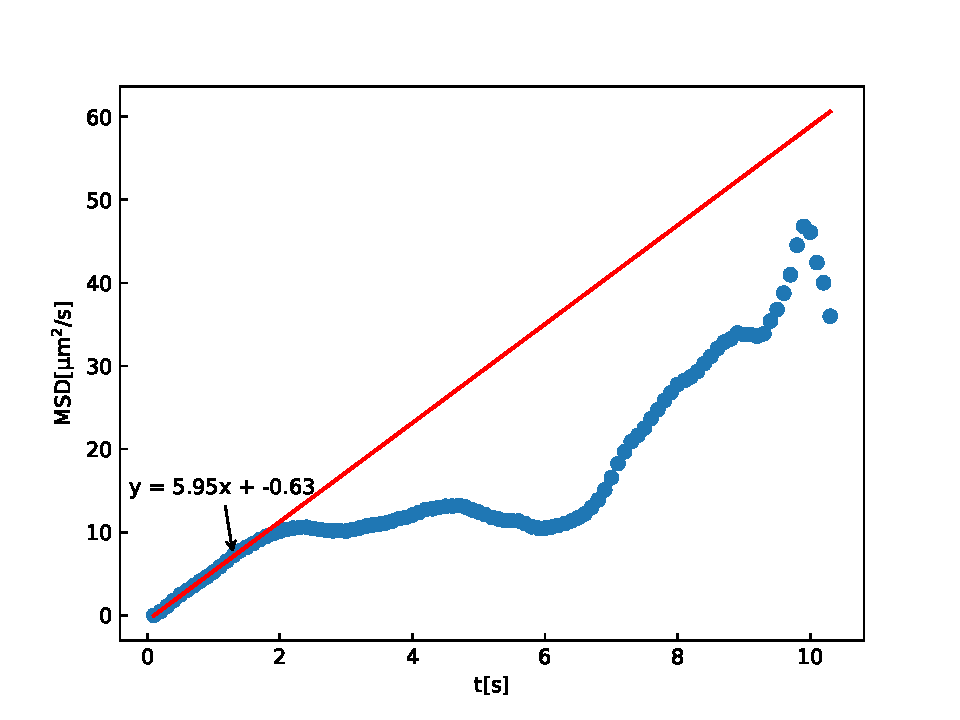
\includegraphics[width=0.7\linewidth]{fig/water_D.pdf}
  \caption{Time variation of MSD of particles in water}
  \label{fig:move_plot}
  \end{figurehere}

  続いて、Fig.6にPEG15\%のMSDの時間依存性を示した。\\
  0〜1.8s近辺の間は、線形的に増加している。この時の傾きを求めると、$5.95 \text{μm}^2/\text{s}^2$となった。\\
  これより、÷8をして拡散係数を求めると、$7.4375×10^{-13} \text{m}^2/\text{s}^2$となった。\\

\section{\textrm{Discussion}}
\subsection*{課題}
以下、温度を$T = 293 \, \mathrm{K}$であると仮定する。\\\\
1. 一次元エネルギー等分配則を用いて、アルゴン原子、半径$1 \, \text{μ}\mathrm{m}$のポリスチレン粒子、ゴルフボールに対して、熱運動の特徴的な速さを計算により見積もる。

一次元エネルギー等分配則は:
\begin{equation}
\frac{1}{2} m\langle v^2 \rangle = \frac{kT}{2}
\end{equation}
であるから、それぞれの質量がわかればボルツマン定数$k$と温度$T$より速さは:
\begin{equation}
\langle v \rangle = \sqrt{\frac{kT}{m}}
\end{equation}
と求められる。ボルツマン定数$k$は :
\begin{equation}
k \approx 1.38 \times 10^{-23}
\end{equation}
である。

アルゴン原子、ポリスチレン粒子、ゴルフボールの半径と質量はそれぞれ、表1に示した。\\

\begin{center}
\begin{table}[ht]
\caption{球体と見積もった場合の、半径と質量の値}
\centering
\begin{tabular}{cccc}
  \hline
   & アルゴン原子 & ポリスチレン粒子 & ゴルフボール \\
  \hline
  半径 [m] & $7.1 \times 10^{-8}$ & $1.0 \times 10^{-6}$ & $2.1 \times 10^{-2}$ \\
  \hline
  質量 [kg] & $6.6 \times 10^{-26}$ & $3.1 \times 10^{-15}$ & $4.6 \times 10^{-2}$ \\
  \hline
\end{tabular}
\end{table}
\end{center}

これらの値を用いて、速さを計算すると、アルゴン原子、ポリスチレン粒子、ゴルフボールの熱運動の速さはそれぞれ次のように見積もられる:
\begin{equation}
  \langle v_{\text{Ar}} \rangle \approx 2.5 \times 10^2
  \end{equation}
  \begin{equation}
  \langle v_{\text{ポリ}} \rangle \approx 1.1 \times 10^{-3}
  \end{equation}
  \begin{equation}
  \langle v_{\text{ゴルフ}} \rangle \approx 3.0 \times 10^{-10}
  \end{equation}

  2. 式$\langle x^2(t) \rangle = {2kT}/{m\gamma^2 (\gamma t - 1 + e^{-\gamma t})}$に関して、短時間極限($\gamma t \ll 1$)を考え、その物理的解釈を考察する。また、
  アルゴン原子、半径$1\mu m$のポリスチレン粒子、ゴルフボールに対して、それぞれ緩和
  時間$1/\gamma$を計算する。
  
  $\langle x^2(t) \rangle = {2kT}/{m\gamma^2 (\gamma t - 1 + e^{-\gamma t})}$は短時間極限($\gamma t \ll 1$)であれば、次のようにテイラー展開できる:
  \begin{equation}
  \langle x^2(t) \rangle = \frac{2kT}{m\gamma^2} \gamma^2 t^2 = \frac{kTt^2}{m}
  \end{equation}
  
  変位の変数は時間$t$だけなので、すなわち、平均二乗変位は時間についての
  二次関数で与えられることが分かる。
  また、変位は:
  \begin{equation}
  \langle x(t) \rangle = \sqrt{\frac{kT}{m}}t
  \end{equation}
  であらわされる。この結果は、変位を微分すると、速度の式(2)になることと一致する。\\
  
  緩和時間$1/\gamma$は式$m\gamma = 6\pi\eta a$より計算することができる:
  \begin{equation}
  \frac{1}{\gamma} = \frac{m}{6\pi\eta a}
  \end{equation}

  純水の場合($\eta = 0.00089$)を考えれば、表1の値を代入して、
  アルゴン原子の緩和時間は:
  \begin{equation}
    5.5 \times 10^{-17}
    \end{equation}
    ポリスチレン粒子の緩和時間は:
    \begin{equation}
    1.8 \times 10^{-7}
    \end{equation}
    ゴルフボールの緩和時間は:
    \begin{equation}
    1.3 \times 10^{2}
    \end{equation}
    となった。\\

    \subsection*{ボルツマン定数の導出}
    拡散係数の測定結果は、表2のようになった。\\
    \begin{center}
      \begin{table}[ht]
      \caption{拡散係数の測定結果}
      \centering
      \begin{tabular}{cccc}
        \hline
         & PEG15\% & PEG30\% & 純水 \\
        \hline
        拡散係数 [$10^{-13} \text{m}^2/\text{s}^2$] & $0.864$ & $0.100$ & $7.44$ \\
        \hline
      \end{tabular}
      \end{table}
      \end{center}
      これらの値を用いて、ボルツマン定数を求める。\\
      アインシュタイン・ストークスの関係式:
    \begin{equation}
      k = \frac{6D\pi\eta a}{T}
      \end{equation}
      を用いると、ボルツマン定数はそれぞれ、表3のように求められた。\\
      \begin{center}
        \begin{table}[ht]
        \caption{求めたボルツマン定数}
        \centering
        \begin{tabular}{cccc}
          \hline
           & PEG15\% & PEG30\% & 純水 \\
          \hline
          拡散係数 [$10^{-23}$] & $3.53$ & $1.42$ & $1.59$ \\
          \hline
        \end{tabular}
        \end{table}
        \end{center}
\section{\textrm{Conclusion}}


\begin{thebibliography}{文献数}
\bibitem{ID} 参考文献の名前・著者1
\bibitem{ID2} 参考文献の名前・著者2
\bibitem{ID3} 参考文献の名前・著者3
\end{thebibliography}

\end{document}